\chapter*{Actividades}

\section*{Consideraciones/Suposiciones}

El modelado de todo el proyecto se realizó bajo las siguientes suposiciones acerca del comportamiento del semáforo de calle:
\begin{itemize}
    \item Los cambios de estado se dan como greenyellow, yellowred, redgreen.
    \item Los semáforos de una misma calle están sincronizados, por lo tanto, solo se controla el comportamiento de los semáforos en la calle Norte-Sur y los semáforos de la calle Este-Oeste.
\end{itemize}


%--------------------------------------------------------------------

\section*{Ejercicio 1}
\textit{\textbf{Consigna:} Modelo base cíclico fijo. Implementar en NuSMV un modelo donde los semáforos cambian de fase únicamente basados en temporizadores (sin considerar demanda). Elegir valores adecuados para Tverde = 10 ticks, Tamarillo = 3 ticks. Verificar si las propiedades se cumplen.}

Para resolver esta consigna, además de las suposiciones generales para todos los modelos, también se consideraron la siguientes suposiciones:
\begin{enumerate}
    \item El tiempo máximo TM es la suma de los tiempos $T_{green}$ y $T_{yellow}$. Entonces un ciclo dura $TM = 10+3 = 13\ ticks$.
    \item Nunca los semáforos de ambas calles estarán en rojo en simultáneo
\end{enumerate}

\begin{lstlisting}[language=NuSMV]
    MODULE semaforo(cross, id, TM, TYellow, TGreen)
    VAR
    state : {red, yellow, green};
    time : 0..TM;
    ASSIGN
    init(state) := case
        cross =  id : green;
        TRUE: red;
    esac;
    init(time) := case
        cross = id : 0;
        cross != id : TM;
    esac;
    next(state) := case
        state = green & cross = id  : yellow;
        state = yellow & cross = id  : red;
        state = red & next(cross) = id : green;
        TRUE: red;
    esac;

    next(time) := case
        next(state) = green : 0;
        next(state) = yellow : TGreen;
        next(state) = red : TM;
    esac;


    MODULE main
    VAR
    semaforo_NS : semaforo(cross, ns, TM, TYellow, TGreen);
    semaforo_OE : semaforo(cross, oe, TM, TYellow, TGreen);
    cross : {ns, oe};

    ASSIGN
    init(cross) := {ns, oe};
    next(cross) := case
        cross = ns & semaforo_NS.state = yellow : oe;
        cross = oe & semaforo_OE.state = yellow : ns;
        TRUE : cross;
    esac;

    DEFINE
    TYellow := 3;
    TGreen := 10;
    TM := TYellow + TGreen;  -- El tiempo total del ciclo

    -- phi 1: Los semaforos de direcciones cruzadas no pueden estar en green simultaneamente.
    LTLSPEC NAME ambosSemaforosIguales := G(semaforo_NS.state != semaforo_OE.state); --verifica que ambos semaforos no sean rojos

    -- phi 2: El yellow debe durar exactamente TYellow y no debe saltarse.
    LTLSPEC NAME spec2 := G(semaforo_NS.time = TGreen -> X(semaforo_NS.time = TM) & G (semaforo_NS.state = green -> X(semaforo_NS.state = yellow))) & G(semaforo_OE.time = TGreen -> X(semaforo_OE.time = TM) & G (semaforo_OE.state = green -> X(semaforo_OE.state = yellow)));

    LTLSPEC NAME spec2_2 := G(semaforo_NS.state = yellow -> semaforo_NS.time = TGreen & X(semaforo_NS.state = red -> semaforo_NS.time = TM)); --Sabemos que TM es TYellow -- phi 4: El tiempo de green no debe exceder un maximo Tmax (ej. 30 segundos).

    -- Q4
    LTLSPEC NAME noExcede := G(TGreen < TM);

    -- phi 5: Siempre es posible que algun semaforo este en green
    CTLSPEC NAME posibleVerde := AG( EF (semaforo_NS.state = green | semaforo_OE.state = green));

\end{lstlisting}


%--------------------------------------------------------------------


\begin{figure}[H]
    \centering
    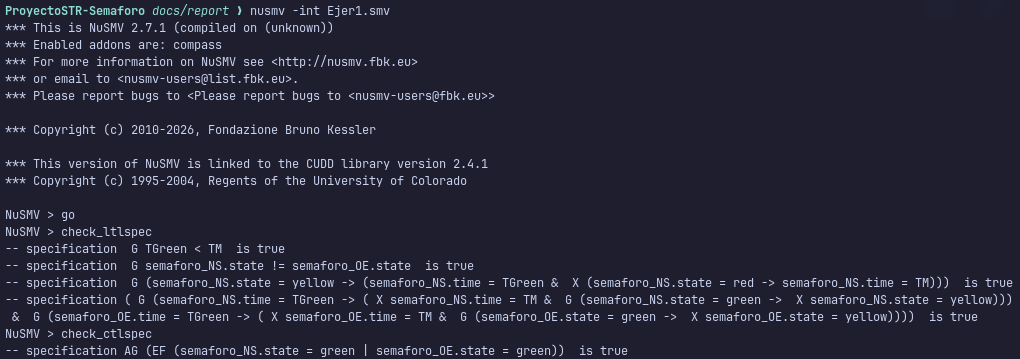
\includegraphics[width=\textwidth]{../resources/resultado_ej1.png}
    \caption{Resultados de verificación para el Ejercicio 1.}
\end{figure}


\section*{Ejercicio 2}

\textit{\textbf{Consigna:} Modificar el modelo para que el semáforo se mantenga en verde si hay demanda en su mismo sentido, hasta un máximo de $T_{max} = 15\ ticks$. Si no hay demanda en el sentido actual pero sí en el otro, el cambio de fase ocurre inmediatamente (respetando el amarillo). Verificar las propiedades nuevamente y si alguna falla, explicar por qué.}

Para esta actividad, se mantuvo la suposición 2 del modelo base, se cambió el nombre de la variable $T_{green}$ por $T_{greenMin}$ y se agregó la variable $T_{greenMax} = 15$.
Se asumio lo siguiente:

\begin{itemize}
    \item El tiempo máximo $TM$ será la suma de $T_{greenMax}$ y $T_{yellow}$.
Tiempo en el que el semáforo está en amarillo ahora crece por ticks, para eso se agrego dentro del modulo semaforo una variable timeyellow que se incrementa en 1 por cada transicion mientras sea menor que $T_{Yellow}$.
    \item Como el tiempo en amarillo cambio, ya no basta con colocar en la transición de cross que cuando el semaforo este en amarillo se realiza el cambio, sino que ahora se debe tener en cuenta que el semaforo estuvo en amarillo un intervalo de tiempo igual a $T_{Yellow}$.
\end{itemize}


\begin{lstlisting}[language=NuSMV, caption={Modelo con demanda y extensión inteligente}]
MODULE semaforo(cross, id, TM, TGreenMin, TYellow, TGreenMax)
VAR
    state : {red, yellow, green};
    time : 0..TM;
    demand : boolean;
    timeyellow : 0..TYellow;

ASSIGN
init(state) := case
    cross =  id : green;
    TRUE: red;
esac;

init(time) := case
    cross = id : 0;
    cross != id : TM;
esac;

init(timeyellow) := 0;

next(state) := case
    next(cross) = id: case --Si el semaforo tiene el turno
        state = green : case --Si actualmente esta en verde
            next(time) < TGreenMin : green; --Que siga en verde si aun no ha pasado un tiempo minimo
            demand & next(time) < TGreenMax : green; --Si paso el tiempo minimo entonces que siga siempre y cuando no pase de un tiempo maximo 
            TRUE : yellow; --Si llego al tiempo maximo o no hay demanda, entonces que pase a amarillo
        esac;
        state = yellow : case --Si actualmente esta en amarillo
            next(timeyellow) < TYellow : yellow; --Que siga en amarillo mientras no haya superado los 3 segundos
            TRUE: red; --Una vez superado llegue a los 3 segundos, entonces que pase a rojo
        esac;
        state = red : green; --Si es su turno y esta rojo, entonces significa que ahora debe cambiar a verde
    esac;
    TRUE : red; --Si no es su turno, entonces debe mantenerse en rojo
esac;

next(time) := case
    next(cross) = id : case --Si es su turno
        state = red: 0; --Si esta en rojo, eso significa que hay que empezar el semaforo
        time < TM: time + 1; --En otro caso, hay que incrementarlo
        TRUE : TM; --Cuando llegue a TM, que se mantenga ahi
    esac;
    TRUE: TM; --Si no es su turno, entonces dejarlo en el tiempo maximo
esac;

next(demand) := case 

    next(state) = green  | next(state) = yellow : {TRUE, FALSE}; --Si esta en verde o amarillo, entonces puede seguir la demanda o apagarse
    demand = FALSE : {TRUE, FALSE}; --Si no hay demanda, en cualquier momento puede llegar autos o seguir sin demanda
    TRUE : TRUE; --Si el siguiente estado no es verde y hay demanda, entonces esta no va a desaparecer
esac;

next(timeyellow) := case
    state = yellow & timeyellow < TYellow : timeyellow + 1;
    TRUE : 0;
esac;

MODULE main
VAR
    cross : {ns, oe};
    semaforo_NS : semaforo(cross, ns, TM, TGreenMin, TYellow,TGreenMax);
    semaforo_OE : semaforo(cross, oe, TM, TGreenMin, TYellow,TGreenMax);
    
ASSIGN
    init(cross) := {ns, oe};
    next(cross) := case
        cross = ns & semaforo_NS.state = yellow & next(semaforo_NS.timeyellow) = TYellow : oe; --Si el semaforo esta en amarillo y ya termino su tiempo, ahora le toca empezar al otro semaforo
        cross = oe & semaforo_OE.state = yellow & next(semaforo_OE.timeyellow) = TYellow : ns; --Si el semaforo esta en amarillo y ya termino su tiempo, ahora le toca empezar al otro semaforo
        TRUE : cross;
    esac;
DEFINE
    TYellow := 3; 
    TGreenMax := 15;
    TGreenMin := 10;
    TM := TYellow + TGreenMax;  -- El tiempo total del ciclo

-- phi 1: Los semaforos de direcciones cruzadas no pueden estar en green simultaneamente.
LTLSPEC NAME ambosSemaforosIguales := G(semaforo_NS.state != semaforo_OE.state); -- Verifica que ambos semaforos no sean rojos

-- phi 2: El yellow debe durar exactamente TYellow y no debe saltarse.
-- LTLSPEC NAME spec2 := G((semaforo_NS.time >= TGreenMin & semaforo_NS.state = yellow) -> X(semaforo_NS.time <= TM & semaforo_NS.time >= (TYellow + TGreenMin))) | G((semaforo_NS.time >= TGreenMin & semaforo_NS.state = yellow) -> X(semaforo_NS.time <= TM & semaforo_NS.time >= (TYellow + TGreenMax)))
LTLSPEC NAME spec2 := G(F(semaforo_NS.timeyellow = TYellow) & F(semaforo_OE.timeyellow = TYellow))

-- phi 3: Si hay vehiculos esperando en una direccion y el semaforo esta rojo, eventualmente se pondra verde.
LTLSPEC NAME demandaYRojo := G((semaforo_NS.demand & semaforo_NS.state = red -> F (semaforo_NS.state = green)) & (semaforo_OE.demand & semaforo_OE.state = red -> F (semaforo_OE.state = green)));

-- phi 4: El tiempo de verde no debe exceder un maximo Tmax (ej. 30 segundos).
LTLSPEC NAME noExcede := G(!(semaforo_NS.state = green &  semaforo_NS.time = TGreenMax) & !(semaforo_OE.state = green &  semaforo_OE.time = TGreenMax)); 

-- phi 5: Siempre es posible que algun semaforo este en green
CTLSPEC NAME posibleVerde := AG( EF (semaforo_NS.state = green | semaforo_OE.state = green));
\end{lstlisting}

%--------------------------------------------------------------------


\begin{figure}[H]
    \centering
    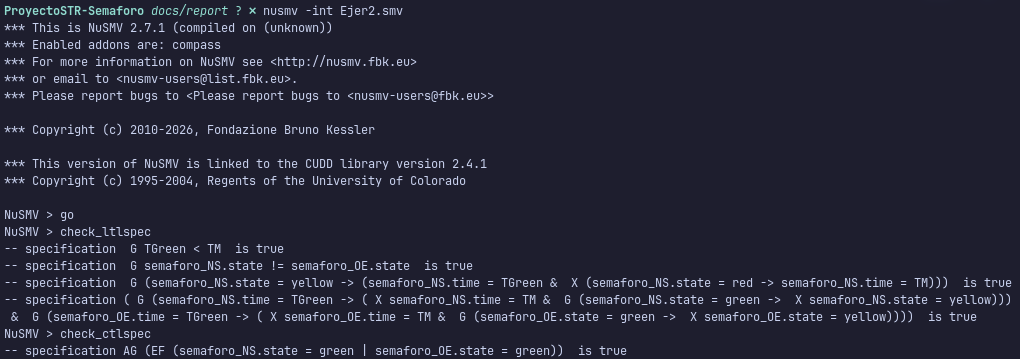
\includegraphics[width=\textwidth]{../resources/resultado_ej2.png}
    \caption{Resultados de verificación para el Ejercicio 2.}
\end{figure}


\section*{Ejercicio 3}
\textit{\textbf{Consigna:} Modificar el modelo para poder verificar que el tiempo máximo de espera para un vehículo (desde que llega hasta que obtiene verde) no supere L = 20 ticks. Especificar esta propiedad en CTL y verificarla.}

En esta actividad, además de las suposiciones base, también se asumió lo siguiente:

\begin{enumerate}
    \item Como en todo momento hay un semaforo en verde o amarillo, solo contabilizamos el tiempo que lleva esperando un auto en el otro semaforo. Es decir, se cuentan cuantos ticks lleva la variable “demand” en true en el semáforo que no tiene aún el turno.
\end{enumerate}


\begin{lstlisting}[language=NuSMV, caption={Modelo con tiempo de espera}]
MODULE semaforo(cross, id, TM, TGreenMin, TYellow, TGreenMax)
VAR
    state : {red, yellow, green};
    time : 0..TM;
    demand : boolean;
    timeyellow : 0..TYellow;

ASSIGN
init(state) := case
    cross =  id : green;
    TRUE: red;
esac;

init(time) := case
    cross = id : 0;
    cross != id : TM;
esac;

init(timeyellow) := 0;

next(state) := case
    next(cross) = id: case --Si el semaforo tiene el turno
        state = green : case --Si actualmente esta en verde
            next(time) < TGreenMin : green; --Que siga en verde si aun no ha pasado un tiempo minimo
            demand & next(time) < TGreenMax : green; --Si paso el tiempo minimo entonces que siga siempre y cuando no pase de un tiempo maximo 
            TRUE : yellow; --Si llego al tiempo maximo o no hay demanda, entonces que pase a amarillo
        esac;
        state = yellow : case --Si actualmente esta en amarillo
            next(timeyellow) < TYellow : yellow; --Que siga en amarillo mientras no haya superado los 3 segundos
            TRUE: red; --Una vez superado llegue a los 3 segundos, entonces que pase a rojo
        esac;
        state = red : green; --Si es su turno y esta rojo, entonces significa que ahora debe cambiar a verde
    esac;
    TRUE : red; --Si no es su turno, entonces debe mantenerse en rojo
esac;

next(time) := case
    next(cross) = id : case --Si es su turno
        state = red: 0; --Si esta en rojo, eso significa que hay que empezar el semaforo
        time < TM: time + 1; --En otro caso, hay que incrementarlo
        TRUE : TM; --Cuando llegue a TM, que se mantenga ahi
    esac;
    TRUE: TM; --Si no es su turno, entonces dejarlo en el tiempo maximo
esac;

next(demand) := case 
    next(state) = green | next(state) = yellow : {TRUE, FALSE}; --Si esta en verde o en amarillo, entonces puede seguir la demanda o apagarse
    demand = FALSE : {TRUE, FALSE}; --Si no hay demanda, en cualquier momento puede llegar autos o seguir sin demanda
    TRUE : TRUE; --Si el siguiente estado no es verde y hay demanda, entonces esta no va a desaparecer
esac;

next(timeyellow) := case
    state = yellow & timeyellow < TYellow : timeyellow + 1;
    TRUE : 0;
esac;

MODULE main
VAR
    cross : {ns, oe};
    semaforo_NS : semaforo(cross, ns, TM, TGreenMin, TYellow,TGreenMax);
    semaforo_OE : semaforo(cross, oe, TM, TGreenMin, TYellow,TGreenMax);
    t_car_arrival : 0..L;
    
ASSIGN
    init(cross) := {ns, oe};
    init(t_car_arrival) := 0;
    next(cross) := case
        cross = ns & semaforo_NS.state = yellow & next(semaforo_NS.timeyellow) = TYellow : oe; --Si el semaforo esta en amarillo y ya termino su tiempo, ahora le toca empezar al otro semaforo
        cross = oe & semaforo_OE.state = yellow & next(semaforo_OE.timeyellow) = TYellow : ns; --Si el semaforo esta en amarillo y ya termino su tiempo, ahora le toca empezar al otro semaforo
        TRUE : cross;
    esac;
    next(t_car_arrival) := case
        
        cross = ns : case
            next(cross) = oe : 0;
            t_car_arrival = L : L; -- Esto le indica al compilador (NuSMV) que la variable no supera el limite
            semaforo_OE.demand : t_car_arrival + 1;
            TRUE: 0; 
        esac;
        
        cross = oe: case
            next(cross) = ns : 0;
            t_car_arrival = L : L; -- Esto le indica al compilador (NuSMV) que la variable no supera el limite
            semaforo_NS.demand : t_car_arrival + 1;
            TRUE: 0;
        esac;
        
    esac;
    
DEFINE
    TYellow := 3; 
    TGreenMax := 15;
    TGreenMin := 10;
    TM := TYellow + TGreenMax;  -- El tiempo total del ciclo
    L := 21;

-- phi 1: Los semaforos de direcciones cruzadas no pueden estar en green simultaneamente.
LTLSPEC NAME ambosSemaforosIguales := G(semaforo_NS.state != semaforo_OE.state); -- Verifica que ambos semaforos no sean rojos

-- phi 2: El yellow debe durar exactamente TYellow y no debe saltarse.
-- LTLSPEC NAME spec2 := G((semaforo_NS.time >= TGreenMin & semaforo_NS.state = yellow) -> X(semaforo_NS.time <= TM & semaforo_NS.time >= (TYellow + TGreenMin))) | G((semaforo_NS.time >= TGreenMin & semaforo_NS.state = yellow) -> X(semaforo_NS.time <= TM & semaforo_NS.time >= (TYellow + TGreenMax)))
LTLSPEC NAME spec2 := G(F(semaforo_NS.timeyellow = TYellow) & F(semaforo_OE.timeyellow = TYellow))

-- phi 3: Si hay vehiculos esperando en una direccion y el semaforo esta rojo, eventualmente se pondra verde.
LTLSPEC NAME demandaYRojo := G((semaforo_NS.demand & semaforo_NS.state = red -> F (semaforo_NS.state = green)) & (semaforo_OE.demand & semaforo_OE.state = red -> F (semaforo_OE.state = green)));

-- phi 4: El tiempo de verde no debe exceder un maximo Tmax (ej. 30 segundos).
LTLSPEC NAME noExcede := G(!(semaforo_NS.state = green &  semaforo_NS.time = TGreenMax) & !(semaforo_OE.state = green &  semaforo_OE.time = TGreenMax)); 

-- phi 5: Siempre es posible que algun semaforo este en green
CTLSPEC NAME posibleVerde := AG( EF (semaforo_NS.state = green | semaforo_OE.state = green));

-- El tiempo de espera nunca debe exceder 20 ticks
CTLSPEC NAME tiempoEspMenor20 := AG (t_car_arrival <= 20);
\end{lstlisting}

%--------------------------------------------------------------------


\begin{figure}[H]
    \centering
    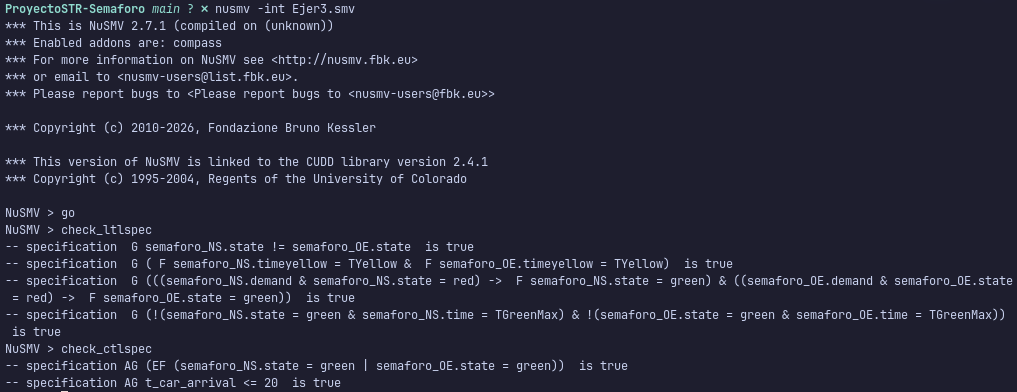
\includegraphics[width=\textwidth]{../resources/resultado_ej3.png}
    \caption{Resultados de verificación para el Ejercicio 3.}
\end{figure}


\section*{Ejercicio 4}

\textit{\textbf{Consigna:} Incorporar al modelo los botones peatonales. Si el botón peatonal es presionado, lo cual puede ocurrir en cualquier momento, el semáforo debe dar verde peatonal (simulado como una fase especial donde ambos semáforos están en rojo) dentro de los siguientes $10\ \text{ticks}$.}

Para el semáforo peatonal:
\begin{itemize}
    \item Al presionarse el botón para dar cruce peatonal, instantáneamente el semáforo de calle que tenga el cruce (semáforo en $state\ =\ green$) realiza el cambio de estado $green \rightarrow yellow$, respetando la cantidad de ticks en la que el mismo debe permanecer en $yellow$, para luego realizar el cambio de estado $yellow \rightarrow wed$. A partir de este momento ambos semáforos de calle permanecen en red durante $10\ ticks$, que es la cantidad de tiempo que el semáforo peatonal permite el cruce. Luego de que finalice el tiempo de cruce del semáforo peatonal, el cruce se le devuelve al semáforo que estaba en $green$ previo a que se presione el botón de cruce peatonal.
\end{itemize}

\begin{lstlisting}[language=NuSMV, caption={Modelo con botón peatonal}]
MODULE semaforo(cross, id, TM, TGreenMin, TYellow, TGreenMax, walker_press)
VAR
    state : {red, yellow, green};
    time : 0..TM;
    demand : boolean;
    timeyellow : 0..TYellow;

ASSIGN
init(state) := case
    cross =  id : green;
    TRUE: red;
esac;

init(time) := case
    cross = id : 0;
    cross != id : TM;
esac;

init(timeyellow) := 0;

next(state) := case
    state = green & walker_press : yellow; --Si esta en verde y se aprieta el boton peatonan entonces que pase automaticamente amarillo
    state = red & walker_press : red; --Si esta en rojo y se apreto el boton entonces que se mantenga el semaforo en rojo
    next(cross) = id: case --Si el semaforo tiene el turno
        state = green : case --Si actualmente esta en verde
            next(time) < TGreenMin : green; --Que siga en verde si aun no ha pasado un tiempo minimo
            demand & next(time) < TGreenMax : green; --Si paso el tiempo minimo entonces que siga siempre y cuando no pase de un tiempo maximo 
            TRUE : yellow; --Si llego al tiempo maximo o no hay demanda, entonces que pase a amarillo
        esac;
        state = yellow : case --Si actualmente esta en amarillo
            next(timeyellow) < TYellow : yellow; --Que siga en amarillo mientras no haya superado los 3 segundos
            TRUE: red; --Una vez superado llegue a los 3 segundos, entonces que pase a rojo
        esac;
        state = red : green; --Si es su turno y esta rojo, entonces significa que ahora debe cambiar a verde
    esac;
    TRUE : red; --Si no es su turno, entonces debe mantenerse en rojo
esac;

next(time) := case
    next(cross) = id : case --Si es su turno
        state = red: 0; --Si esta en rojo, eso significa que hay que empezar el semaforo
        time < TM: time + 1; --En otro caso, hay que incrementarlo
        TRUE : TM; --Cuando llegue a TM, que se mantenga ahi
    esac;
    TRUE: TM; --Si no es su turno, entonces dejarlo en el tiempo maximo
esac;

next(demand) := case 
    next(state) = green | next(state) = yellow : {TRUE, FALSE}; --Si esta en verde o en amarillo, entonces puede seguir la demanda o apagarse
    demand = FALSE : {TRUE, FALSE}; --Si no hay demanda, en cualquier momento puede llegar autos o seguir sin demanda
    TRUE : TRUE; --Si el siguiente estado no es verde y hay demanda, entonces esta no va a desaparecer
esac;

next(timeyellow) := case
    state = yellow & timeyellow < TYellow : timeyellow + 1;
    TRUE : 0;
esac;

MODULE main
VAR
    cross : {ns, oe}; --Variable que indica de que semaforo es el turno
    semaforo_NS : semaforo(cross, ns, TM, TGreenMin, TYellow, TGreenMax, walker_press); --Modulo del semaforo NS
    semaforo_OE : semaforo(cross, oe, TM, TGreenMin, TYellow, TGreenMax, walker_press); --Modulo del semaforo OE
    t_car_arrival : 0..L; --Tiempo maximo que lleva esperando un auto
    t_walker_cross : 0..P; --Tiempo que llevan los dos semaforos en rojo
    walker_press : boolean; --Variable que controla si se apreto el boton peatonal

ASSIGN
    init(cross) := {ns, oe};
    init(t_car_arrival) := 0;
    init(t_walker_cross) := 0;
    init(walker_press) := FALSE;
    
    next(cross) := case
        cross = ns & semaforo_NS.state = yellow & next(semaforo_NS.timeyellow) = TYellow : oe; --Si el semaforo esta en amarillo y ya termino su tiempo, ahora le toca empezar al otro semaforo
        cross = oe & semaforo_OE.state = yellow & next(semaforo_OE.timeyellow) = TYellow : ns; --Si el semaforo esta en amarillo y ya termino su tiempo, ahora le toca empezar al otro semaforo
        TRUE : cross;
    esac;
    next(t_car_arrival) := case
        
        cross = ns : case
            next(cross) = oe : 0;
            t_car_arrival = L : L; -- Restriccion impuesta para que el sistema (NuSMV) entienda que la variable no supera L
            semaforo_OE.demand : t_car_arrival + 1;
            TRUE: 0; 
        esac;
        
        cross = oe: case
            next(cross) = ns : 0;
            t_car_arrival = L : L; -- Restriccion impuesta para que el sistema (NuSMV) entienda que la variable no supera L
            semaforo_NS.demand : t_car_arrival + 1;
            TRUE: 0;
        esac;
    esac;

    next(walker_press) := case
        !walker_press : {TRUE, FALSE}; -- Si el boton no esta presionado, puede pasar a estar presionado o no en el siguiente estado
        next(t_walker_cross) = P: FALSE; -- Si pasaron los 10 seg en el que ambos semaforos estaban en rojo, entonces se le quita el paso al peaton
        TRUE: TRUE;
    esac;

    next(t_walker_cross) := case 
        t_walker_cross = P : P; -- Restriccion impuesta para que el sistema (NuSMV) entienda que la variable no supera P
        walker_press & semaforo_NS.state = semaforo_OE.state : t_walker_cross + 1;
        TRUE : 0;
    esac;
    
DEFINE
    TYellow := 3; --Tiempo que estara en amarillo el semaforo
    TGreenMax := 15; -- Tiempo maximo del semaforo verde si hay demanda
    TGreenMin := 10; -- Tiempo minimo del semaforo verde con o sin demanda
    TM := TYellow + TGreenMax;  -- El tiempo total del ciclo
    L := 21; -- Tiempo que no debe exceder un auto en espera
    P := 10; -- Tiempo que tienen los peatones para pasar


-- phi 1: Los semaforos de direcciones cruzadas no pueden estar en green simultaneamente.
LTLSPEC NAME ambosSemaforosIguales := !G(semaforo_NS.state = green & semaforo_OE.state = green);

-- phi 2: El yellow debe durar exactamente TYellow y no debe saltarse.
-- LTLSPEC NAME spec2 := G((semaforo_NS.time >= TGreenMin & semaforo_NS.state = yellow) -> X(semaforo_NS.time <= TM & semaforo_NS.time >= (TYellow + TGreenMin))) | G((semaforo_NS.time >= TGreenMin & semaforo_NS.state = yellow) -> X(semaforo_NS.time <= TM & semaforo_NS.time >= (TYellow + TGreenMax)))
LTLSPEC NAME spec2 := G(F(semaforo_NS.timeyellow = TYellow) & F(semaforo_OE.timeyellow = TYellow))

-- phi 3: Si hay vehiculos esperando en una direccion y el semaforo esta rojo, eventualmente se pondra verde.
LTLSPEC NAME demandaYRojo := G((semaforo_NS.demand & semaforo_NS.state = red -> F (semaforo_NS.state = green)) & (semaforo_OE.demand & semaforo_OE.state = red -> F (semaforo_OE.state = green)));

-- phi 4: El tiempo de verde no debe exceder un maximo Tmax (ej. 30 segundos).
LTLSPEC NAME noExcede := G(!(semaforo_NS.state = green &  semaforo_NS.time = TGreenMax) & !(semaforo_OE.state = green &  semaforo_OE.time = TGreenMax)); 

-- phi 5: Siempre es posible que algun semaforo este en green
CTLSPEC NAME posibleVerde := AG( EF (semaforo_NS.state = green | semaforo_OE.state = green));

-- El tiempo de espera nunca debe exceder 20 ticks
CTLSPEC NAME tiempoEspMenor20 := AG (t_car_arrival <= 20);

\end{lstlisting}

%--------------------------------------------------------------------


\begin{figure}[H]
    \centering
    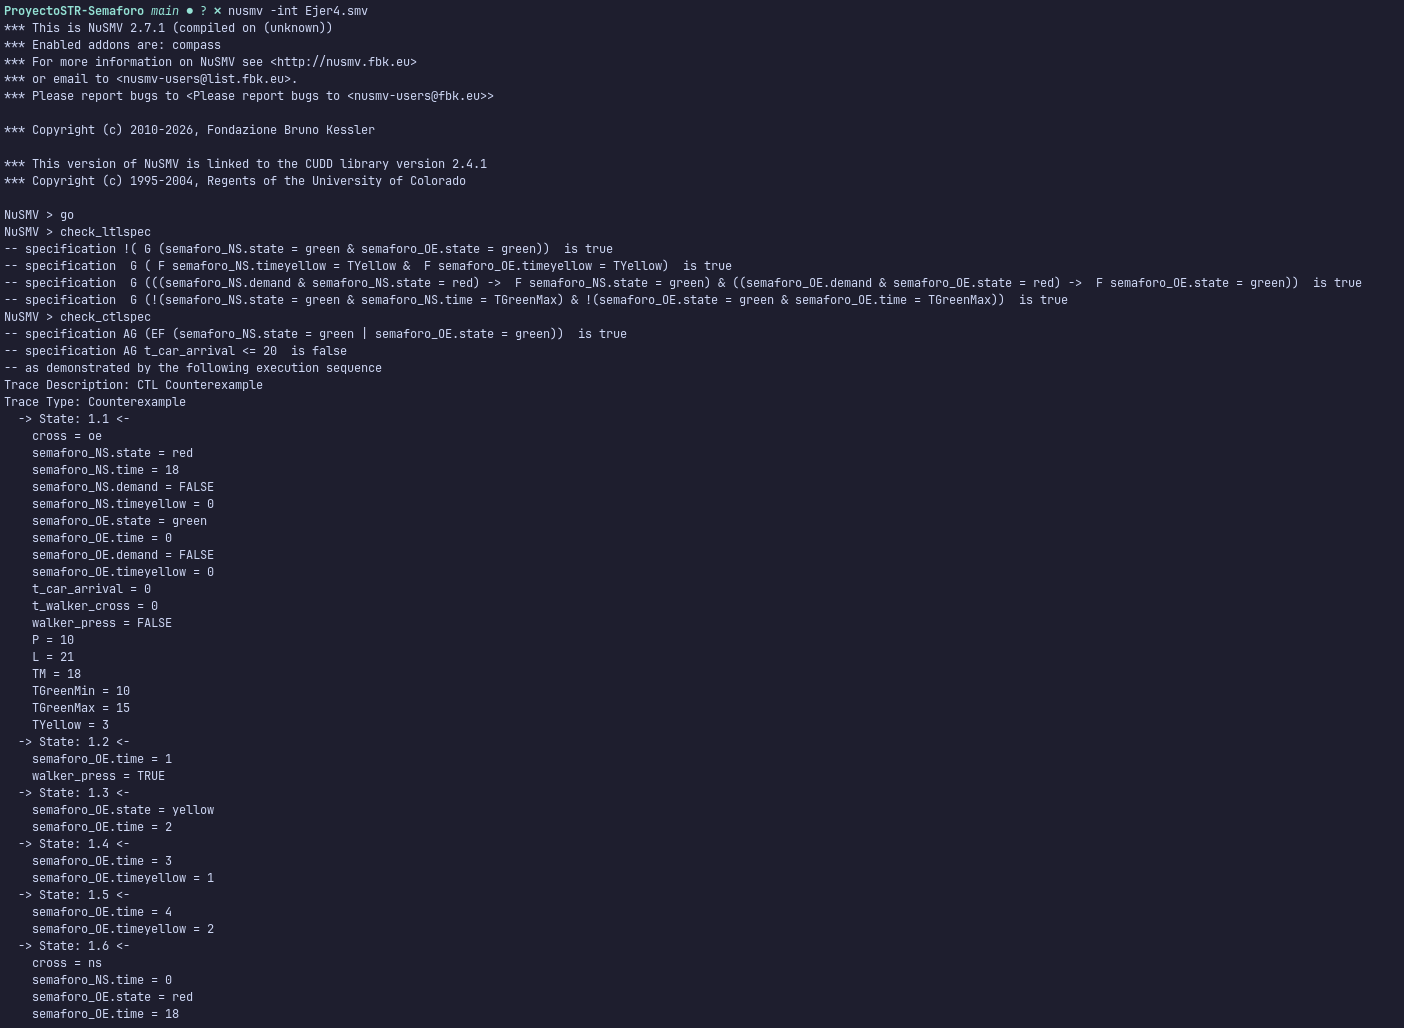
\includegraphics[width=0.8\textwidth]{../resources/resultado_ej4_1.png}
    \caption{Resultados de verificación para el Ejercicio 4 (Parte 1).}
\end{figure}
\begin{figure}[H]
    \centering
    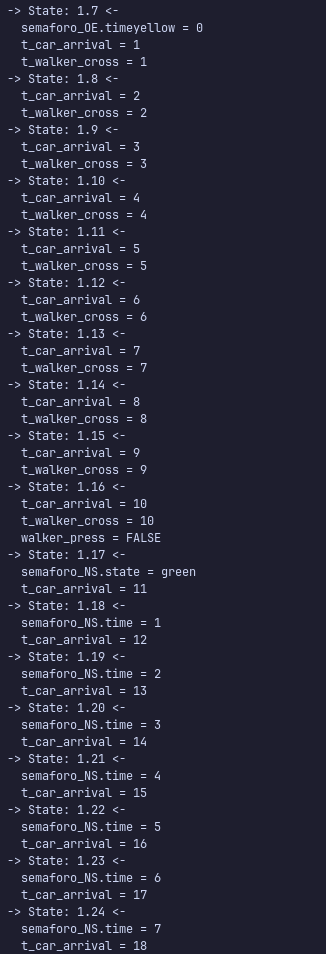
\includegraphics[width=0.5\textwidth]{../resources/resultado_ej4_2.png}
    \caption{Resultados de verificación para el Ejercicio 4 (Parte 2).}
\end{figure}
\begin{figure}[H]
    \centering
    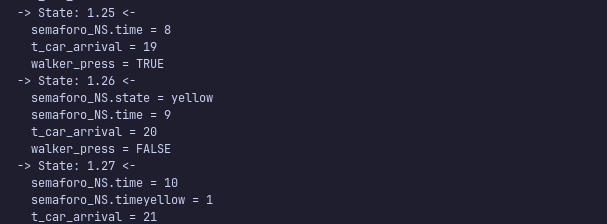
\includegraphics[width=0.8\textwidth]{../resources/resultado_ej4_3.png}
    \caption{Resultados de verificación para el Ejercicio 4 (Parte 3).}
\end{figure}


\section*{Ejercicio 5}
\textit{\textbf{Consigna:} Modificar el modelo para introducir errores deliberados que violen cada una de las propiedades establecidas. Analizar el contraejemplo generado por NuSMV.}

Consideraciones que tuvimos para realizar los contraejemplos:

\begin{itemize}
    \item Usar un error para violar multiples propiedades.
    \item Insertar múltiples errores que rompan múltiples propiedades en un mismo código en vez de crear modelos separados para romper las propiedades de manera individual. Igualmente, debido a la imposibilidad de violar la propiedad 1 y 5 al mismo tiempo, se realizaron 2 modelos con errores.
\end{itemize}
\begin{lstlisting}[language=NuSMV, caption={Modelo con errores introducidos para violar specs 1, 2 y 3}]
-- Para violar las propiedades 1, 2 y 3
MODULE semaforo(cross, id, TM, TGreenMin, TYellow, TGreenMax, walker_press)
VAR
    state : {red, yellow, green};
    time : 0..TM;
    demand : boolean;
    timeyellow : 0..TYellow;

ASSIGN
init(state) := case
    cross =  id : green;
    TRUE: red;
esac;

init(time) := case
    cross = id : 0;
    cross != id : TM;
esac;

init(timeyellow) := 0;

next(state) := case
    state = green & walker_press : yellow; --Si esta en verde y se aprieta el boton peatonan entonces que pase automaticamente amarillo
    state = red & walker_press : red; --Si esta en rojo y se apreto el boton entonces que se mantenga el semaforo en rojo
    next(cross) = id: case --Si el semaforo tiene el turno
        state = green : case --Si actualmente esta en verde
            next(time) < TGreenMin : green; --Que siga en verde si aun no ha pasado un tiempo minimo
            demand & next(time) < TGreenMax : green; --Si paso el tiempo minimo entonces que siga siempre y cuando no pase de un tiempo maximo 
            TRUE : yellow; --Si llego al tiempo maximo o no hay demanda, entonces que pase a amarillo
        esac;
        state = yellow : case --Si actualmente esta en amarillo
            next(timeyellow) < TYellow : yellow; --Que siga en amarillo mientras no haya superado los 3 segundos
            TRUE: red; --Una vez superado llegue a los 3 segundos, entonces que pase a rojo
        esac;
        state = red : green; --Si es su turno y esta rojo, entonces significa que ahora debe cambiar a verde
    esac;
    TRUE : red; --Si no es su turno, entonces debe mantenerse en rojo
esac;

next(time) := case
    next(cross) = id : case --Si es su turno
        state = red: 0; --Si esta en rojo, eso significa que hay que empezar el semaforo
        time < TM: time + 1; --En otro caso, hay que incrementarlo
        TRUE : TM; --Cuando llegue a TM, que se mantenga ahi
    esac;
    TRUE: TM; --Si no es su turno, entonces dejarlo en el tiempo maximo
esac;

next(demand) := case 
    next(state) = green | next(state) = yellow : {TRUE, FALSE}; --Si esta en verde o en amarillo, entonces puede seguir la demanda o apagarse
    demand = FALSE : {TRUE, FALSE}; --Si no hay demanda, en cualquier momento puede llegar autos o seguir sin demanda
    TRUE : TRUE; --Si el siguiente estado no es verde y hay demanda, entonces esta no va a desaparecer
esac;

next(timeyellow) := case
    state = yellow & timeyellow < TYellow : timeyellow + 1;
    TRUE : 0;
esac;

MODULE main
VAR
    cross : {ns, oe}; --Variable que indica de que semaforo es el turno
    semaforo_NS : semaforo(cross, ns, TM, TGreenMin, TYellow, TGreenMax, walker_press); --Modulo del semaforo NS
    semaforo_OE : semaforo(cross, oe, TM, TGreenMin, TYellow, TGreenMax, walker_press); --Modulo del semaforo OE
    t_car_arrival : 0..L; --Tiempo maximo que lleva esperando un auto
    t_walker_cross : 0..P; --Tiempo que llevan los dos semaforos en rojo
    walker_press : boolean; --Variable que controla si se apreto el boton peatonal

ASSIGN
    init(cross) := {ns, oe};
    init(t_car_arrival) := 0;
    init(t_walker_cross) := 0;
    init(walker_press) := FALSE;
    
    -- Aqui se introdujo error, modificando el proximo estado para el cruce, haciendo que den todas las especificaciones faltas, excepto \phi_5
    next(cross) := case
        cross = ns: oe; --CAMBIO: Siempre estan alternando los semaforos
        cross = oe: ns; --CAMBIO: Siempre estan alternando los semaforos
        TRUE : cross;
    esac;
    next(t_car_arrival) := case
        
        cross = ns : case
            next(cross) = oe : 0;
            t_car_arrival = L : L; -- Restriccion impuesta para que el sistema (NuSMV) entienda que la variable no supera L
            semaforo_OE.demand : t_car_arrival + 1;
            TRUE: 0; 
        esac;
        
        cross = oe: case
            next(cross) = ns : 0;
            t_car_arrival = L : L; -- Restriccion impuesta para que el sistema (NuSMV) entienda que la variable no supera L
            semaforo_NS.demand : t_car_arrival + 1;
            TRUE: 0;
        esac;
    esac;

    next(walker_press) := case
        !walker_press : {TRUE, FALSE}; -- Si el boton no esta presionado, puede pasar a estar presionado o no en el siguiente estado
        next(t_walker_cross) = P: FALSE; -- Si pasaron los 10 seg en el que ambos semaforos estaban en rojo, entonces se le quita el paso al peaton
        TRUE: TRUE;
    esac;

    next(t_walker_cross) := case 
        t_walker_cross = P : P; -- Restriccion impuesta para que el sistema (NuSMV) entienda que la variable no supera P
        walker_press & semaforo_NS.state = semaforo_OE.state : t_walker_cross + 1;
        TRUE : 0;
    esac;
    
DEFINE
    TYellow := 3; --Tiempo que estara en amarillo el semaforo
    TGreenMax := 15; -- Tiempo maximo del semaforo verde si hay demanda
    TGreenMin := 10; -- Tiempo minimo del semaforo verde con o sin demanda
    TM := TYellow + TGreenMax;  -- El tiempo total del ciclo
    L := 21; -- Tiempo que no debe exceder un auto en espera
    P := 10; -- Tiempo que tienen los peatones para pasar


-- phi 1: Los semaforos de direcciones cruzadas no pueden estar en green simultaneamente.
LTLSPEC NAME ambosSemaforosIguales := G(semaforo_NS.state = green & semaforo_OE.state = green);

-- phi 2: El yellow debe durar exactamente TYellow y no debe saltarse.
-- LTLSPEC NAME spec2 := G((semaforo_NS.time >= TGreenMin & semaforo_NS.state = yellow) -> X(semaforo_NS.time <= TM & semaforo_NS.time >= (TYellow + TGreenMin))) | G((semaforo_NS.time >= TGreenMin & semaforo_NS.state = yellow) -> X(semaforo_NS.time <= TM & semaforo_NS.time >= (TYellow + TGreenMax)))
LTLSPEC NAME spec2 := G(F(semaforo_NS.timeyellow = TYellow) & F(semaforo_OE.timeyellow = TYellow))

-- phi 3: Si hay vehiculos esperando en una direccion y el semaforo esta rojo, eventualmente se pondra verde.
LTLSPEC NAME demandaYRojo := G((semaforo_NS.demand & semaforo_NS.state = red -> F (semaforo_NS.state = green)) & (semaforo_OE.demand & semaforo_OE.state = red -> F (semaforo_OE.state = green)));

-- phi 4: El tiempo de verde no debe exceder un maximo Tmax (ej. 30 segundos).
LTLSPEC NAME noExcede := G(!(semaforo_NS.state = green &  semaforo_NS.time = TGreenMax) & !(semaforo_OE.state = green &  semaforo_OE.time = TGreenMax)); 

-- phi 5: Siempre es posible que algun semaforo este en green
CTLSPEC NAME posibleVerde := AG( EF (semaforo_NS.state = green | semaforo_OE.state = green));

-- El tiempo de espera nunca debe exceder 20 ticks
CTLSPEC NAME tiempoEspMenor20 := AG (t_car_arrival <= 20);

-- 
\end{lstlisting}

\begin{lstlisting}[language=NuSMV, caption={Modelo con errores introducidos para violar specs 4 y 5}]
-- Para violar las propiedades 4 y 5
MODULE semaforo(cross, id, TM, TGreenMin, TYellow, TGreenMax, walker_press)
VAR
    state : {red, yellow, green};
    time : 0..TM;
    demand : boolean;
    timeyellow : 0..TYellow;

ASSIGN
init(state) := case
    cross =  id : green;
    TRUE: red;
esac;

init(time) := case
    cross = id : 0;
    cross != id : TM;
esac;

init(timeyellow) := 0;

next(state) := case
    state = green & walker_press : yellow; --Si esta en verde y se aprieta el boton peatonan entonces que pase automaticamente amarillo
    state = red & walker_press : red; --Si esta en rojo y se apreto el boton entonces que se mantenga el semaforo en rojo
    next(cross) = id: case --Si el semaforo tiene el turno
        state = green : case --Si actualmente esta en verde
            next(time) < TGreenMin : green; --CAMBIO: Que siga en verde si aun no ha pasado un tiempo minimo
            demand & next(time) < TM+1: green; --Ahora esta en verde mas de TM ticks
            TRUE : yellow; --Si llego al tiempo maximo o no hay demanda, entonces que pase a amarillo
        esac;
        state = yellow : case --Si actualmente esta en amarillo
            next(timeyellow) < TYellow : yellow; --Que siga en amarillo mientras no haya superado los 3 segundos
            TRUE: red; --Una vez superado llegue a los 3 segundos, entonces que pase a rojo
        esac;
        state = red : red; --CAMBIO: Si esta en rojo nunca cambiara a verde
    esac;
    TRUE : red; --Si no es su turno, entonces debe mantenerse en rojo
esac;

next(time) := case
    next(cross) = id : case --Si es su turno
        state = red: 0; --Si esta en rojo, eso significa que hay que empezar el semaforo
        time < TM: time + 1; --En otro caso, hay que incrementarlo
        TRUE : TM; --Cuando llegue a TM, que se mantenga ahi
    esac;
    TRUE: TM; --Si no es su turno, entonces dejarlo en el tiempo maximo
esac;

next(demand) := case 
    next(state) = green | next(state) = yellow : {TRUE, FALSE}; --Si esta en verde o en amarillo, entonces puede seguir la demanda o apagarse
    demand = FALSE : {TRUE, FALSE}; --Si no hay demanda, en cualquier momento puede llegar autos o seguir sin demanda
    TRUE : TRUE; --Si el siguiente estado no es verde y hay demanda, entonces esta no va a desaparecer
esac;

next(timeyellow) := case
    state = yellow & timeyellow < TYellow : timeyellow + 1;
    TRUE : 0;
esac;

MODULE main
VAR
    cross : {ns, oe}; --Variable que indica de que semaforo es el turno
    semaforo_NS : semaforo(cross, ns, TM, TGreenMin, TYellow, TGreenMax, walker_press); --Modulo del semaforo NS
    semaforo_OE : semaforo(cross, oe, TM, TGreenMin, TYellow, TGreenMax, walker_press); --Modulo del semaforo OE
    t_car_arrival : 0..L; --Tiempo maximo que lleva esperando un auto
    t_walker_cross : 0..P; --Tiempo que llevan los dos semaforos en rojo
    walker_press : boolean; --Variable que controla si se apreto el boton peatonal

ASSIGN
    init(cross) := {ns, oe};
    init(t_car_arrival) := 0;
    init(t_walker_cross) := 0;
    init(walker_press) := FALSE;
    
    next(cross) := case
        cross = ns & semaforo_NS.state = yellow & next(semaforo_NS.timeyellow) = TYellow : oe; --Si el semaforo esta en amarillo y ya termino su tiempo, ahora le toca empezar al otro semaforo
        cross = oe & semaforo_OE.state = yellow & next(semaforo_OE.timeyellow) = TYellow : ns; --Si el semaforo esta en amarillo y ya termino su tiempo, ahora le toca empezar al otro semaforo
        TRUE : cross;
    esac;
    next(t_car_arrival) := case
        
        cross = ns : case
            next(cross) = oe : 0;
            t_car_arrival = L : L; -- Restriccion impuesta para que el sistema (NuSMV) entienda que la variable no supera L
            semaforo_OE.demand : t_car_arrival + 1;
            TRUE: 0; 
        esac;
        
        cross = oe: case
            next(cross) = ns : 0;
            t_car_arrival = L : L; -- Restriccion impuesta para que el sistema (NuSMV) entienda que la variable no supera L
            semaforo_NS.demand : t_car_arrival + 1;
            TRUE: 0;
        esac;
    esac;

    next(walker_press) := case
        !walker_press : {TRUE, FALSE}; -- Si el boton no esta presionado, puede pasar a estar presionado o no en el siguiente estado
        next(t_walker_cross) = P: FALSE; -- Si pasaron los 10 seg en el que ambos semaforos estaban en rojo, entonces se le quita el paso al peaton
        TRUE: TRUE;
    esac;

    next(t_walker_cross) := case 
        t_walker_cross = P : P; -- Restriccion impuesta para que el sistema (NuSMV) entienda que la variable no supera P
        walker_press & semaforo_NS.state = semaforo_OE.state : t_walker_cross + 1;
        TRUE : 0;
    esac;
    
DEFINE
    TYellow := 3; --Tiempo que estara en amarillo el semaforo
    TGreenMax := 15; -- Tiempo maximo del semaforo verde si hay demanda
    TGreenMin := 10; -- Tiempo minimo del semaforo verde con o sin demanda
    TM := TYellow + TGreenMax;  -- El tiempo total del ciclo
    L := 21; -- Tiempo que no debe exceder un auto en espera
    P := 10; -- Tiempo que tienen los peatones para pasar


-- phi 1: Los semaforos de direcciones cruzadas no pueden estar en green simultaneamente.
LTLSPEC NAME ambosSemaforosIguales := G(semaforo_NS.state = green & semaforo_OE.state = green);

-- phi 2: El yellow debe durar exactamente TYellow y no debe saltarse.
-- LTLSPEC NAME spec2 := G((semaforo_NS.time >= TGreenMin & semaforo_NS.state = yellow) -> X(semaforo_NS.time <= TM & semaforo_NS.time >= (TYellow + TGreenMin))) | G((semaforo_NS.time >= TGreenMin & semaforo_NS.state = yellow) -> X(semaforo_NS.time <= TM & semaforo_NS.time >= (TYellow + TGreenMax)))
LTLSPEC NAME spec2 := G(F(semaforo_NS.timeyellow = TYellow) & F(semaforo_OE.timeyellow = TYellow))

-- phi 3: Si hay vehiculos esperando en una direccion y el semaforo esta rojo, eventualmente se pondra verde.
LTLSPEC NAME demandaYRojo := G((semaforo_NS.demand & semaforo_NS.state = red -> F (semaforo_NS.state = green)) & (semaforo_OE.demand & semaforo_OE.state = red -> F (semaforo_OE.state = green)));

-- phi 4: El tiempo de verde no debe exceder un maximo Tmax (ej. 30 segundos).
LTLSPEC NAME noExcede := G(!(semaforo_NS.state = green &  semaforo_NS.time = TGreenMax) & !(semaforo_OE.state = green &  semaforo_OE.time = TGreenMax)); 

-- phi 5: Siempre es posible que algun semaforo este en green
CTLSPEC NAME posibleVerde := AG( EF (semaforo_NS.state = green | semaforo_OE.state = green));

-- El tiempo de espera nunca debe exceder 20 ticks
CTLSPEC NAME tiempoEspMenor20 := AG (t_car_arrival <= 20);
\end{lstlisting}

%--------------------------------------------------------------------


\begin{figure}[H]
    \centering
    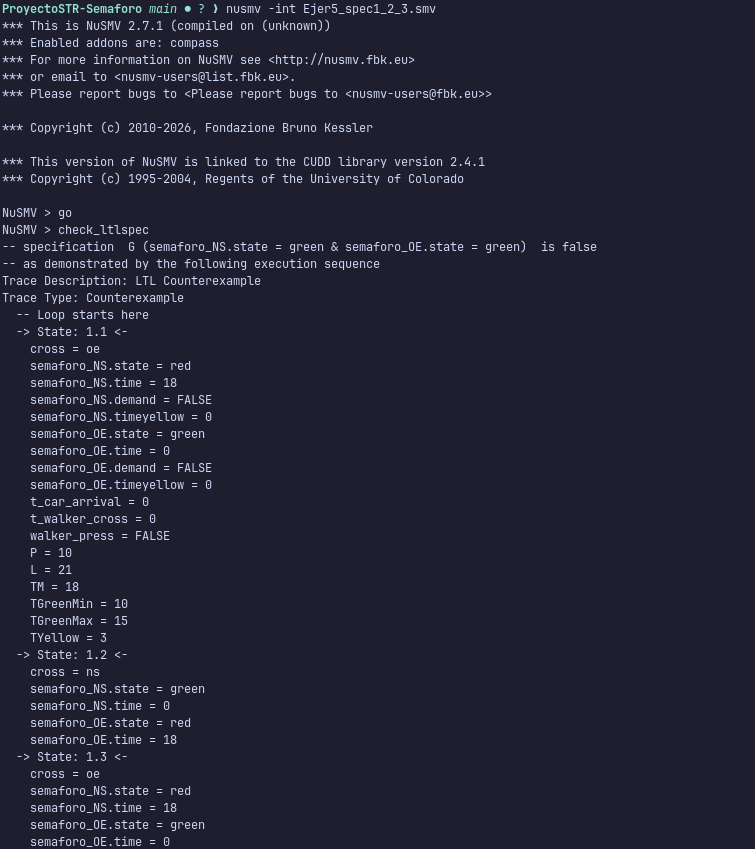
\includegraphics[width=0.8\textwidth]{../resources/resultado_5_1.png}
    \caption{Contraejemplo para la especificación 1.}
\end{figure}
\begin{figure}[H]
    \centering
    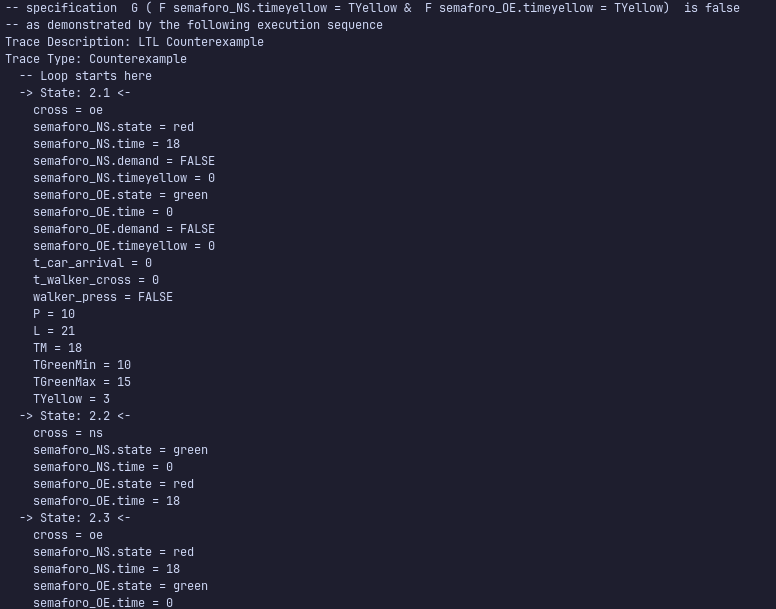
\includegraphics[width=0.8\textwidth]{../resources/resultado_5_2.png}
    \caption{Contraejemplo para la especificación 2.}
\end{figure}
% \begin{figure}[H]
%     \centering
%     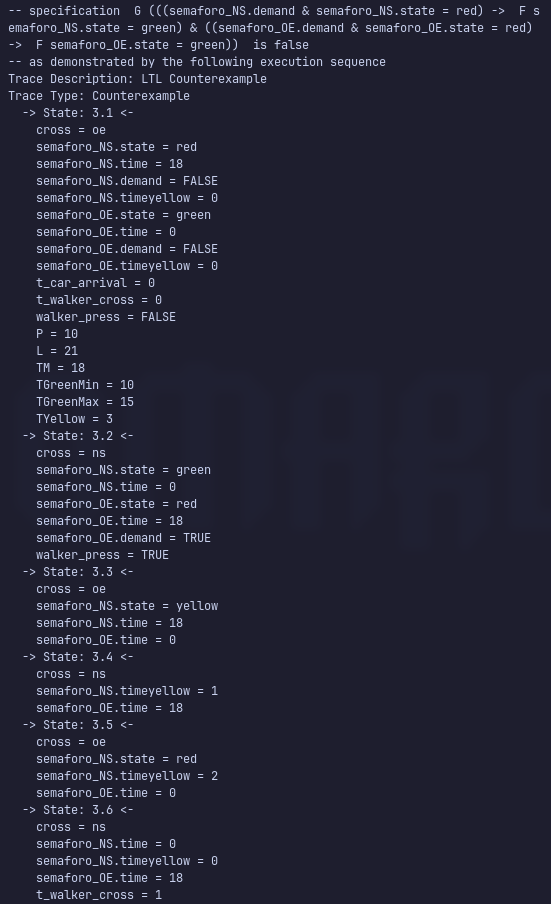
\includegraphics[width=1\textwidth]{../resources/resultado_5_3.png}
%     \caption{Contraejemplo para la especificación 3.}
% \end{figure}
\begin{figure}[H]
    \centering
    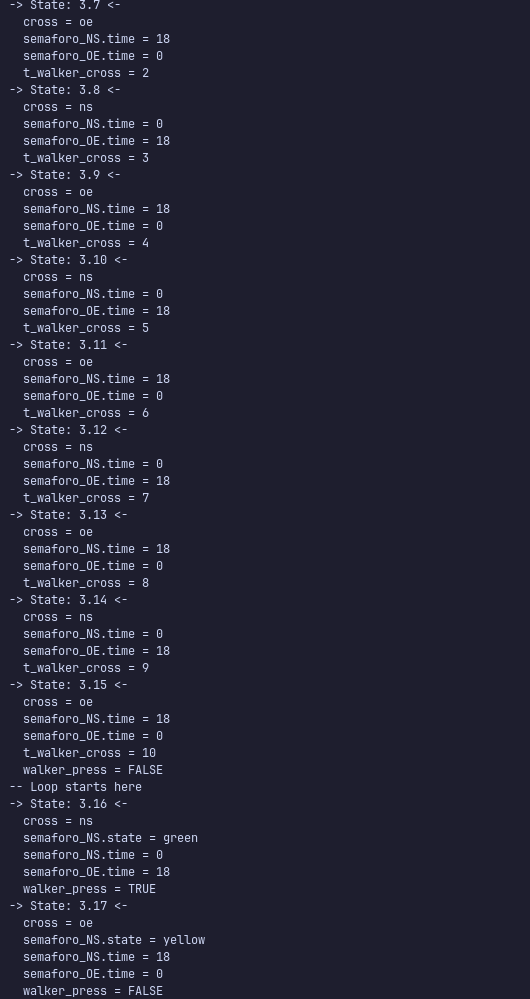
\includegraphics[width=0.8\textwidth]{../resources/resultado_5_4.png}
    \caption{Contraejemplo para la especificación 4.}
\end{figure}
\begin{figure}[H]
    \centering
    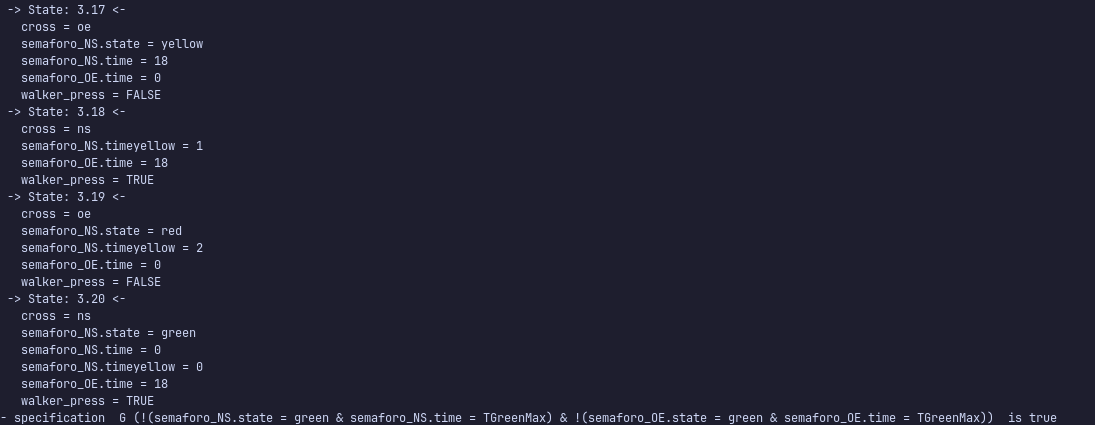
\includegraphics[width=0.8\textwidth]{../resources/resultado_5_5.png}
    \caption{Contraejemplo para la especificación 5.}
\end{figure}
\begin{figure}[H]
    \centering
    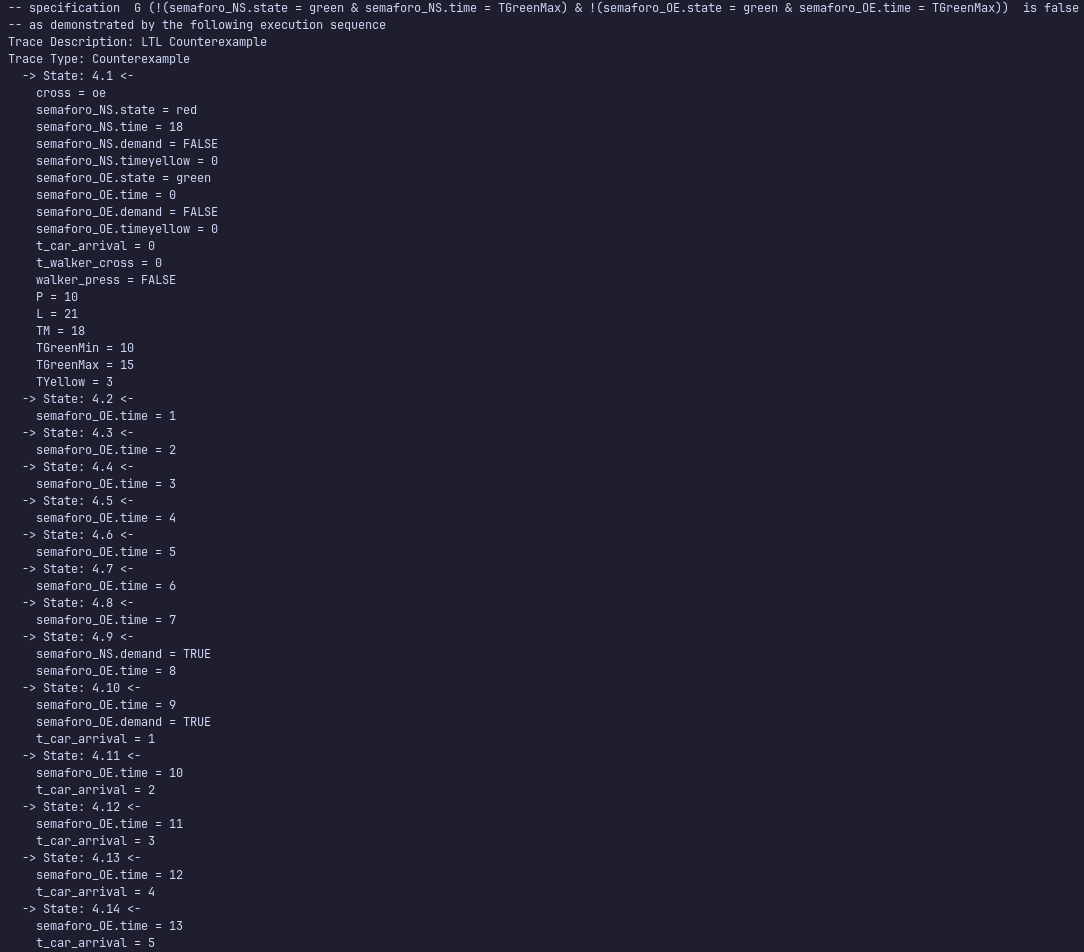
\includegraphics[width=0.8\textwidth]{../resources/resultado_5_6.png}
    \caption{Contraejemplo para la especificación 6.}
\end{figure}
\begin{figure}[H]
    \centering
    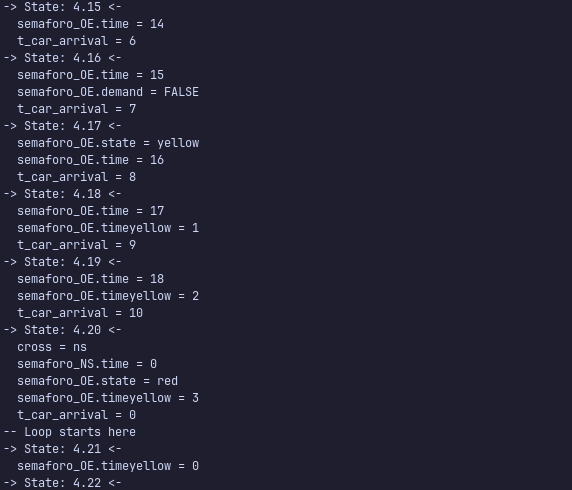
\includegraphics[width=0.8\textwidth]{../resources/resultado_5_7.png}
    \caption{Contraejemplo para la especificación 7.}
\end{figure}
\begin{figure}[H]
    \centering
    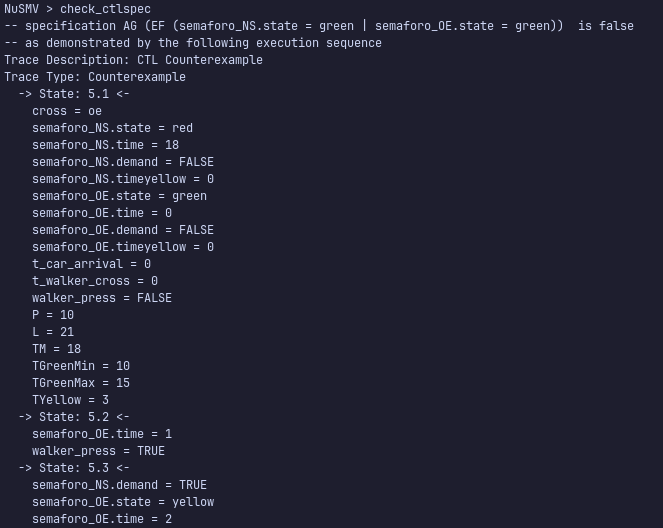
\includegraphics[width=0.8\textwidth]{../resources/resultado_5_8.png}
    \caption{Contraejemplo para la especificación 8.}
\end{figure}


\section*{Ejercicio 6}

\textit{\textbf{Consigna:} Para el modelo final (con demanda y botón peatonal), medir el tiempo de verificación y el número de estados alcanzables usando el comando print reachable states en NuSMV. Comparar con el modelo cíclico fijo. Discutir la complejidad del espacio de estados.}

Para el modelo inicial:

\begin{lstlisting}[language=NuSMV, caption={Resultado de ejecutar el comando \texttt{print\_reachable\_states}}, label=list:reachable_states]
import numpy as np

x  = [0, 1, 2, 3, 4, 5] # assign values to an array
evenSum = evenSummation(x) # call a function

def evenSummation(x):
    evenSum = 0
    n = len(x)
    for i in range(n):
        if np.mod(x[i],2) == 0: # check if a number is even?
            evenSum = evenSum + x[i]
    return evenSum
\end{lstlisting}


%--------------------------------------------------------------------

\section*{Ejercicio 7}

\subsubsection*{¿Por qué es importante verificar propiedades de seguridad en sistemas de tiempo real? Dé un ejemplo concreto diferente al de los semáforos.}

Dado un sistema/realidad a modelar, se requiere que esta tenga un comportamiento particular esperado. De esta manera, al verificar propiedades, validamos que el sistema nunca entrará en un estado no deseado o peligroso (safety). Pero también se debe complementar con las propiedades de vitalidad, para asegurarse de que el sistema progrese, y de Fairness, para evitar ejecuciones irreales.

Por ejemplo, un cajero automático solo puede expulsar dinero si el usuario ingresado dispone del mismo.

\subsubsection*{Explique la diferencia entre CTL y LTL.}

La diferencia entre CTL y LTL, es que el primero se define para árboles de ejecución y el último se define para caminos de ejecución.

\begin{figure}[H]
    \centering
    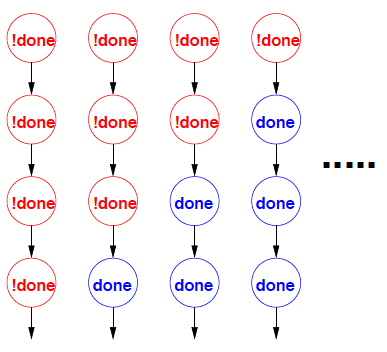
\includegraphics[width=0.4\textwidth]{../resources/LTL.png}
    \caption{LTL}
\end{figure}

\begin{figure}[H]
    \centering
    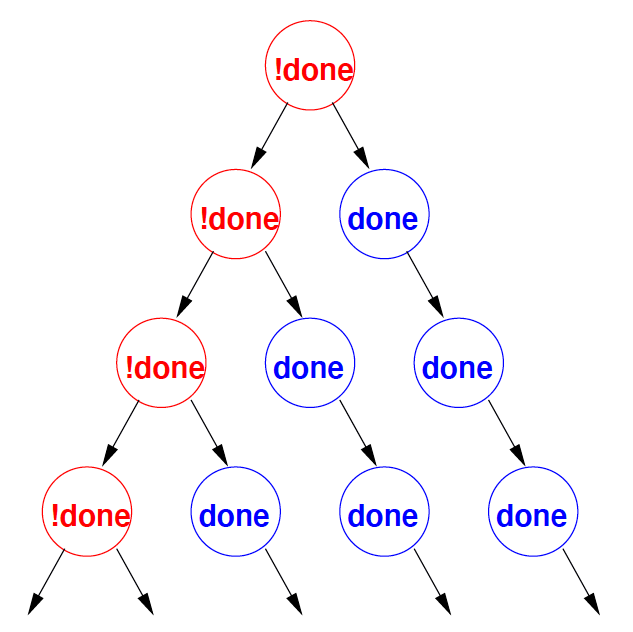
\includegraphics[width=0.4\textwidth]{../resources/CTL.png}
    \caption{CTL}
\end{figure}

Además, el LTL permite expresar cómo evolucionan los estados a lo largo del tiempo en una ejecución y el CTL permite combinar cuantificadores de camino con operadores temporales.

\subsubsection*{¿Cómo modelaría un fallo en el sensor de demanda (ej. sensor siempre activo)? ¿Qué propiedad se violaría?}

Esto podría lograrse agregando una variable \texttt{sensorFail : boolean} que de manera no determinística modele un fallo en el sensor. Luego, en la condición para cambiar el estado del semáforo de \texttt{green} a \texttt{yellow}, modificaría la condición que determina si el semáforo permanece en \texttt{green} si \texttt{demand \& !sensorFail}, para que el semáforo permanezca en \texttt{green}.

De esta manera, independientemente de si hay verdaderamente demanda o no (para un cruce particular), si hay falla de sensor, entonces el semáforo no considera extenderse por demanda.

Considerando de que nos estamos refiriendo a las propiedades especificadas para esta actividad, y no las propiedaes de \textit{safety}, \textit{liveness} y \textit{fairness},inguna propiedad se violaría, siguiendo el modelo completo y el agregando la variable \texttt{sensorFail : boolean}, debido a que:

\begin{enumerate}
    \item La propiedad $\phi_1$ se mantiene ya que este modelo no permite semáforos en verde en simultáneo. Cuando falla un sensor de un semáforo, el semáforo actúa con su tiempo mínimo siempre.
    \item La propiedad $\phi_2$ se sigue cumpliendo ya que el semáforo sigue teniendo su comportamiento normal de \texttt{green $\rightarrow$ yellow $\rightarrow$ red $\rightarrow$ green}, por lo que yellow seguirá tardando Tyellow.
    \item La propiedad $\phi_3$ se mantiene ya que el semáforo sigue teniendo el comportamiento de \texttt{green $\rightarrow$ yellow $\rightarrow$ red $\rightarrow$ green} determinado, por lo que eventualmente ocurrirá el cambio para el otro semáforo.
    \item La propiedad $\phi_4$ se cumple ya que, si no funciona el sensor de demanda, el tiempo verde cumple un tiempo mínimo, por lo que nunca excede el \texttt{TM}.
    \item La propiedad $\phi_5$ se sigue manteniendo ya que, aun si falla algún sensor de demanda, entonces el semáforo aún actúa de manera cíclica y por tanto siempre en algún momento algún semáforo estará en verde.
\end{enumerate}

